\documentclass[
  bibliography=totoc,     % Literatur im Inhaltsverzeichnis
  captions=tableheading,  % Tabellenüberschriften
  titlepage=firstiscover, % Titelseite ist Deckblatt
]{scrartcl}
\usepackage{parskip}
% Paket float verbessern
\usepackage{scrhack}

% Warnung, falls nochmal kompiliert werden muss
\usepackage[aux]{rerunfilecheck}

% deutsche Spracheinstellungen
\usepackage{polyglossia}
\setmainlanguage{german}

% unverzichtbare Mathe-Befehle
\usepackage{amsmath}
% viele Mathe-Symbole
\usepackage{amssymb}
% Erweiterungen für amsmath
\usepackage{mathtools}

% Fonteinstellungen
\usepackage{fontspec}
% Latin Modern Fonts werden automatisch geladen

\usepackage[
  math-style=ISO,    % ┐
  bold-style=ISO,    % │
  sans-style=italic, % │ ISO-Standard folgen
  nabla=upright,     % │
  partial=upright,   % ┘
  warnings-off={           % ┐
    mathtools-colon,       % │ unnötige Warnungen ausschalten
    mathtools-overbracket, % │
  },                       % ┘
]{unicode-math}

% traditionelle Fonts für Mathematik
\setmathfont{Latin Modern Math}
\setmathfont{XITS Math}[range={scr, bfscr}]
\setmathfont{XITS Math}[range={cal, bfcal}, StylisticSet=1]

% Zahlen und Einheiten
\usepackage[
  locale=DE,                 % deutsche Einstellungen
  separate-uncertainty=true, % immer Fehler mit \pm
  per-mode=reciprocal,       % ^-1 für inverse Einheiten
  output-decimal-marker=.,   % . statt , für Dezimalzahlen
]{siunitx}

% chemische Formeln
\usepackage[
  version=4,
  math-greek=default, % ┐ mit unicode-math zusammenarbeiten
  text-greek=default, % ┘
]{mhchem}

% richtige Anführungszeichen
\usepackage[autostyle]{csquotes}

% schöne Brüche im Text
\usepackage{xfrac}

% Standardplatzierung für Floats einstellen
\usepackage{float}
\floatplacement{figure}{htbp}
\floatplacement{table}{htbp}

% Floats innerhalb einer Section halten
\usepackage[
  section, % Floats innerhalb der Section halten
  below,   % unterhalb der Section aber auf der selben Seite ist ok
]{placeins}

% Seite drehen für breite Tabellen
\usepackage{pdflscape}

% Captions schöner machen.
\usepackage[
  labelfont=bf,        % Tabelle x: Abbildung y: ist jetzt fett
  font=small,          % Schrift etwas kleiner als Dokument
  width=0.9\textwidth, % maximale Breite einer Caption schmaler
]{caption}
% subfigure, subtable, subref
\usepackage{subcaption}

% Grafiken können eingebunden werden
\usepackage{graphicx}
% größere Variation von Dateinamen möglich
\usepackage{grffile}

% schöne Tabellen
\usepackage{booktabs}

% Verbesserungen am Schriftbild
\usepackage{microtype}

% Literaturverzeichnis
\usepackage[
  style=numeric,
  sorting=none,
  backend=biber,
]{biblatex}
% Quellendatenbank
\addbibresource{lit.bib}
\addbibresource{programme.bib}

%Biber bringt nichts durcheinander
%\usepackage[sort&compress,numbers]{natbib}

% Hyperlinks im Dokument
\usepackage[
  unicode,        % Unicode in PDF-Attributen erlauben
  pdfusetitle,    % Titel, Autoren und Datum als PDF-Attribute
  pdfcreator={},  % ┐ PDF-Attribute säubern
  pdfproducer={}, % ┘
]{hyperref}
% erweiterte Bookmarks im PDF
\usepackage{bookmark}

% Trennung von Wörtern mit Strichen
\usepackage[shortcuts]{extdash}

% tikzpicture
\usepackage{tikz}
\usetikzlibrary{circuits.ee.IEC}
\usetikzlibrary{positioning}
\tikzset{
  Pfeil/.style={thick,shorten >=#1,shorten <=#1,->,>=latex}, % für Peile
  UPfeil/.style={blue,Pfeil=#1,font={\sffamily\itshape}},% für Spannungspfeile
  IPfeil/.style={red,Pfeil=#1,font={\ttfamily\itshape}} % für Strompfeile
}
%Volt- und Amperemeter festlegen:
\tikzset{circuit declare symbol = Us}
\tikzset{set Us graphic ={draw,generic circle IEC, minimum size=5mm,info=center:Us}}

\tikzset{circuit declare symbol = voltmeter}
\tikzset{set voltmeter graphic ={draw,generic circle IEC, minimum size=5mm,info=center:V}}

\tikzset{circuit declare symbol = ammeter}
\tikzset{set ammeter graphic ={draw,generic circle IEC, minimum size=5mm,info=center:A}}


\tikzset{circuit declare symbol = AC source}
\tikzset{AC source IEC graphic/.style={
    circuit symbol lines,
    circuit symbol size=width 2 height 2,
    shape=generic circle IEC,
    /pgf/generic circle IEC/before background={
    \pgfpathmoveto{\pgfpoint{-0.8pt}{0pt}}
    \pgfpathsine{\pgfpoint{0.4pt}{0.4pt}}
    \pgfpathcosine{\pgfpoint{0.4pt}{-0.4pt}}
    \pgfpathsine{\pgfpoint{0.4pt}{-0.4pt}}
    \pgfpathcosine{\pgfpoint{0.4pt}{0.4pt}}
    \pgfusepath{stroke}
    },
    transform shape, draw
  }
}
\tikzset{circuit ee IEC/.append style=
  {set AC source graphic = AC source IEC graphic}
}

\author{
  Johannes Kollek%
  \texorpdfstring{
    \\
    \href{mailto:johannes.kollek@udo.edu}{johannes.kollek@udo.edu}
  }{}%
  \texorpdfstring{\and}{, }
  Jean-Marco Alameddine%
  \texorpdfstring{
    \\
    \href{mailto:jean-marco.alameddine@udo.edu}{jean-marco.alameddine@udo.edu}
  }{}%
}
\publishers{TU Dortmund – Fakultät Physik}


\subject{Versuchsprotokoll zum Versuch Nr. 302}
\title{Brückenschaltungen}
\date{
  Durchführung: 10.11.2015
}

\begin{document}

\maketitle
%\thispagestyle{empty}
\newpage

\section{Zielsetzung}
Das vorliegene Experiment dient dem Ziel, die Messung unbekannter Widerstäde, Induktivitäten und Kapazitäten mithilfe von Brückenschaltungen anhand mehrerer Beispiele durchzuführen.

\section{Versuchsziel}
\label{sec:Versuchsziel}
Das Ziel des Experiments ist es, die Wellenlänge eines Lasers und die Brechungsindizes zweier Gase mit Hilfe eines Michelson-Interferometers zu bestimmen.

\section{Theorie}
\label{sec:Theorie}

In letzter Zeit ist es Wissenschaftlern gelungen, Gravitationswellen nachzuweisen.
Hierzu wurde ein Michelson-Interferometer benutzt, da es dazu geeignet ist, Wellenlängen, sowie deren absolute Änderung zu messen.
Zusätzlich können auch Brechungsindizes gemessen werden.
Das Michelson-Interferometer selbst stützt sich auf das Interferenzprinzip, auf welches im Folgenden weiter eingegangen wird.\\
\subsection{Interferenz des Lichtes}
Im Allgemeinen kann Licht als elektromagnetische Welle der Form
\begin{equation}
  \vec{E}(x,t) = \vec{E_0}\exp{(i(\vec{k}\vec{x}-\omega t -\delta))}, \label{eqn:1}
\end{equation}
mit Ort $\vec{x}$ und Zeit $t$, sowie Wellenvektor $\vec{k}$, Frequenz $\omega$ und Phasenkonstante $\delta$, angenommen werden, wobei sie sich nur in ihrer Intensität
\begin{equation}
  I = const |\vec{E}|²
\end{equation}
messbar macht.
Da diese elektromagnetischen Wellen den Maxwell-Gleichungen unterliegen, gilt die lineare Superposition, wodurch sich zwei Wellen einfach addieren lassen.
Aus Gründen der Messbarkeit muss hier jedoch auf ein zeitliches Mittel zurückgegriffen werden, wodurch sich für die gesamte Intensität $I_{\text{ges}}$ der Ausdruck
\begin{equation}
  I_{\text{ges}} = \frac{const}{t_2-t_1} \int_{t_1}^{t_2} (|\vec{E_1}+\vec{E_2}|)²(x,t) dt
\end{equation}
ergibt. Dabei muss darauf geachtet werden, dass die Periodendauer $T = 2\pi/\omega$ groß gegenüber der Länge des Messintervalls ist.
Somit ergibt sich für zwei Lichtwellen der Form \eqref{eqn:1}, welche sich nur in ihrer Phase unterscheiden,
\begin{equation}
  I_{\text{ges}} = const \cdot 2\vec{E_0}(1+\cos{\delta_2-\delta_1}).
\end{equation}
Hierbei spiegelt der Cosinus den Interferenzterm wieder.
Erkennbar ist, dass, wenn der Phasenunterschied $(\delta_2-\delta_1)$ ungerade Vielfache von $\pi$ beträgt, es zur Auslöschung der beobachtbaren Intensität führt.
Dies wird als destruktive Interferenz bezeichnet.
Ein Kernkriterium, unter dem Interferenzerscheinungen beobachtbar werden, ist die Kohärenz der beiden Lichtbündel.\\

\subsection{Kohärenz und Kohärenzlänge}
Zwei Wellen sind zueinander zeitlich kohärent, wenn sie, abgesehen von ihrer Phase, zeitlich das selbe Schwingungsmuster in ihrem Zug aufweisen.
Dabei ist auf die Entstehung des Lichtes zu achten:
Licht wird in einem gewissen Zeitfenster von angeregten Atomen emittiert.
Bei mehreren Atomen (im Prinzip Lichtquellen) überlagern sich ihre Wellengruppen.
Hierbei ist zu erwähnen, dass ihre Phasenkonstanten im Allgemeinen statistische Funktionen $\delta(t)$ der Zeit sind.
Demnach können verschieden große bzw. kleine Werte angenommen werden.
Daraus folgt, dass der gemittelte Cosinus der Phasendifferenz,
\begin{equation}
  \frac{1}{t_2-t_1} \int_{t_1}^{t_2} \cos{\delta_2(t)-\delta_1(t)}dt \approx 0,
\end{equation}
nicht mehr beobachtbar ist.
Deswegen ist das Licht zweier unterschiedlicher Lichtquellen allgemein nicht interferenzfähig; es ist inkohärent.\\
Prinzipiell kann das Licht einer einzigen Lichtquelle aufgespalten und wieder zusammengeführt werden, um Interferenzeffekte zu beobachten.
Dabei wird bevorzugt das Licht von Lasern verwendet, da es mit ihnen möglich ist kohärentes Licht zu erzeugen.
Dies ist schematisch in Abbildung \ref{abb:1} dargestellt.
\begin{figure}[H]
  \centering
  \includegraphics[height=4cm]{ressources/spaltung.png}
  \caption{Aufspaltung und Zusammenführung eines Lichtbündels. \cite{Quelle0}}
  \label{abb:1}
\end{figure}
Beträgt die Differenz der beiden Wege nun ungeradzahlige Vielfache der halben Wellenlänge,
\begin{equation}
  \Delta = (2n+1)\frac{\lambda}{2},
\end{equation}
so kommt es erneut zu Auslöschungseffekten am Punkt P.
Wichtig ist zusätzlich noch die Kohärenzlänge $l$.
Da, wie bereits erwähnt, die Emission von Licht in endlichen Zeitabständen $\tau$ stattfindet, haben die Wellenzüge eine endliche Länge.
Wird diese überschritten, überlagern sich am Zusammentreffungspunkt zwei Wellenzüge von unterschiedlichen Emissionsakten, was bei hinreichend großem Wegunterschied zum Verschwinden des Interferenzeffektes führt.
Demnach wird die Kohärenzlänge festgelegt als das Produkt der bei P maximal beobachtbaren Intensitätsmaxima $N$ mit der Wellenlänge $\lambda$ des Lichtes,
\begin{equation}
  l = N\lambda.\\
\end{equation}
Zusätzlich kann die Breite der Lichtquelle zur Verhinderung der Interferenzerscheinungen führen, da das emittierte Licht an verschiedenen Stellen möglicherweise Phasenverschiebungen aufweist, die insgesamt in einer Inkohärenz enden.\\


\subsection{Wellenlängenmessung mittels Interferenz}

Die Quintessenz dieses Abschnittes lautet, dass sich die Wellenlänge einer Lichtquelle über eine Aufspaltung des Lichtes auf verschieden lange Wege, wobei einer um eine Strecke $\Delta l$ variiert wird, und anschließender Zusammenführung der Strahlen durch eine Zählung der entstehenden Interferenzmaxima bestimmen lässt.
Dies genügt der Gleichung
\begin{equation}
  \Delta l = N\frac{\lambda}{2}, \label{eqn:2}
\end{equation}
bei der $N$ die gezählten Interferenzmaxima beschreibt.\\

\subsection{Bestimmung eines Brechungsindex über Interferenz}

Befindet sich die Messapparatur in einem Medium, herrscht auf jeder Wegstrecke der Brechungsindex $n$.
Wird ein anderes Medium der Dicke $b$ einem Strahlengang in den Weg gesetzt, durchläuft das Licht auf diesem Ast eine zusätzliche effektive Weglänge von $b\Delta n$.
Dadurch lässt sich bei bekannter Wellenlänge die Änderung des Brechungsindex $\Delta n$,
\begin{equation}
  b\Delta n = N\frac{\lambda}{2}, \label{eqn:3}
\end{equation}
beschreiben.
Zur Berechnung des Brechungsindex unter Normalbedingungen wird die Formel
\begin{equation}
  n(p_0,T_0) = 1 +\Delta n(\Delta p) \frac{T}{T_0}\frac{p_0}{\Delta p}
\end{equation}
verwendet, bei der $p_0$ den Normaldruck und $T_0$ die Normaltemperatur beschreibt.
Wird diese Formel durch den Ausdruck (\ref{eqn:3}) ergänzt ergibt sich
\begin{equation}
  n(p_0,T_0) = 1 +\frac{N \lambda}{2b} \frac{T}{T_0}\frac{p_0}{\Delta p}, \label{eqn:soso}
\end{equation}
wobei $\lambda$ die Wellenlänge des Lasers und $b$ die Länge des Gasbehälters ist, welchen das Laserlicht passiert.





% 2x2 Plot
% \begin{figure*}
%     \centering
%     \begin{subfigure}[b]{0.475\textwidth}
%         \centering
%         \includegraphics[width=\textwidth]{Abbildungen/Schaltung1.pdf}
%         \caption[]%
%         {{\small Schaltung 1.}}
%         \label{fig:Schaltung1}
%     \end{subfigure}
%     \hfill
%     \begin{subfigure}[b]{0.475\textwidth}
%         \centering
%         \includegraphics[width=\textwidth]{Abbildungen/Schaltung2.pdf}
%         \caption[]%
%         {{\small Schaltung 2.}}
%         \label{fig:Schaltung2}
%     \end{subfigure}
%     \vskip\baselineskip
%     \begin{subfigure}[b]{0.475\textwidth}
%         \centering
%         \includegraphics[width=\textwidth]{Abbildungen/Schaltung4.pdf}    % Zahlen vertauscht ... -.-
%         \caption[]%
%         {{\small Schaltung 3.}}
%         \label{fig:Schaltung3}
%     \end{subfigure}
%     \quad
%     \begin{subfigure}[b]{0.475\textwidth}
%         \centering
%         \includegraphics[width=\textwidth]{Abbildungen/Schaltung3.pdf}
%         \caption[]%
%         {{\small Schaltung 4.}}
%         \label{fig:Schaltung4}
%     \end{subfigure}
%     \caption[]
%     {Ersatzschaltbilder der verschiedenen Teilaufgaben.}
%     \label{fig:Schaltungen}
% \end{figure*}

\subsection{Durchführung}
\label{sec:durchführung}

\section{Diskussion}
\label{sec:Diskussion}



Der aus Plot \ref{plot:6} bestimmte Quotient aus der Planckschen Konstante und der Elementarladung lautet
\begin{align*}
  \left(\frac{h}{e_0}\right)_{\text{gem}} = \input{build/a_6.tex}.
\end{align*}
Verglichen mit dem Literaturwert \cite{Konstanten},
\begin{align*}
  \left(\frac{h}{e_0}\right)_{\text{lit}} = \input{build/a_lit.tex},
\end{align*}
ergibt sich eine prozentuale Abweichung von
\begin{align*}
  \increment{\left(\frac{h}{e_0}\right)} = \input{build/abw_he.tex}.
\end{align*}
Die aus jenem Plot berechnete Austrittsarbeit beträgt
\begin{align*}
  A = \input{build/ak.tex}.
\end{align*}
Es fallen jedoch zwei Sonderheiten auf.
Zunächst sieht es so aus, als würden die Punkte des Plots eher einen quadratisch ansteigenden Trend verfolgen, welcher die Theorie wiederlegen wiederlegen würde.
Die berechnete Steigung bestätigt die Theorie wiederrum, was darauf schließen lässt, dass die bestimmten Punkte durch eine unglückliche Messdatenaufnahme vom wahren Wert abweichen.
Zum Beispiel könnte dies an der geringen Intensität und oder Fokussierung der Spektrallinien liegen. Exemplarisch lässt sich hier die blaugrüne Linie herauspicken, da sie durch eine sehr schwache Intensität gekennzeichnet ist.
Zum anderen war es schwierig die ultraviolette Linie aufzunehmen, da diese nur auf dem floureszierenden Schirm zu sehen ist.\\
Insgesamt lässt sich die Theorie zum Photoeffekt bestätigen, jedoch laden gewisse Messungenauigkeiten eher zu einem sogenannten vorsichtigen Genuss ein.



\section{Anhang}
\begin{figure}[H]
  \centering
  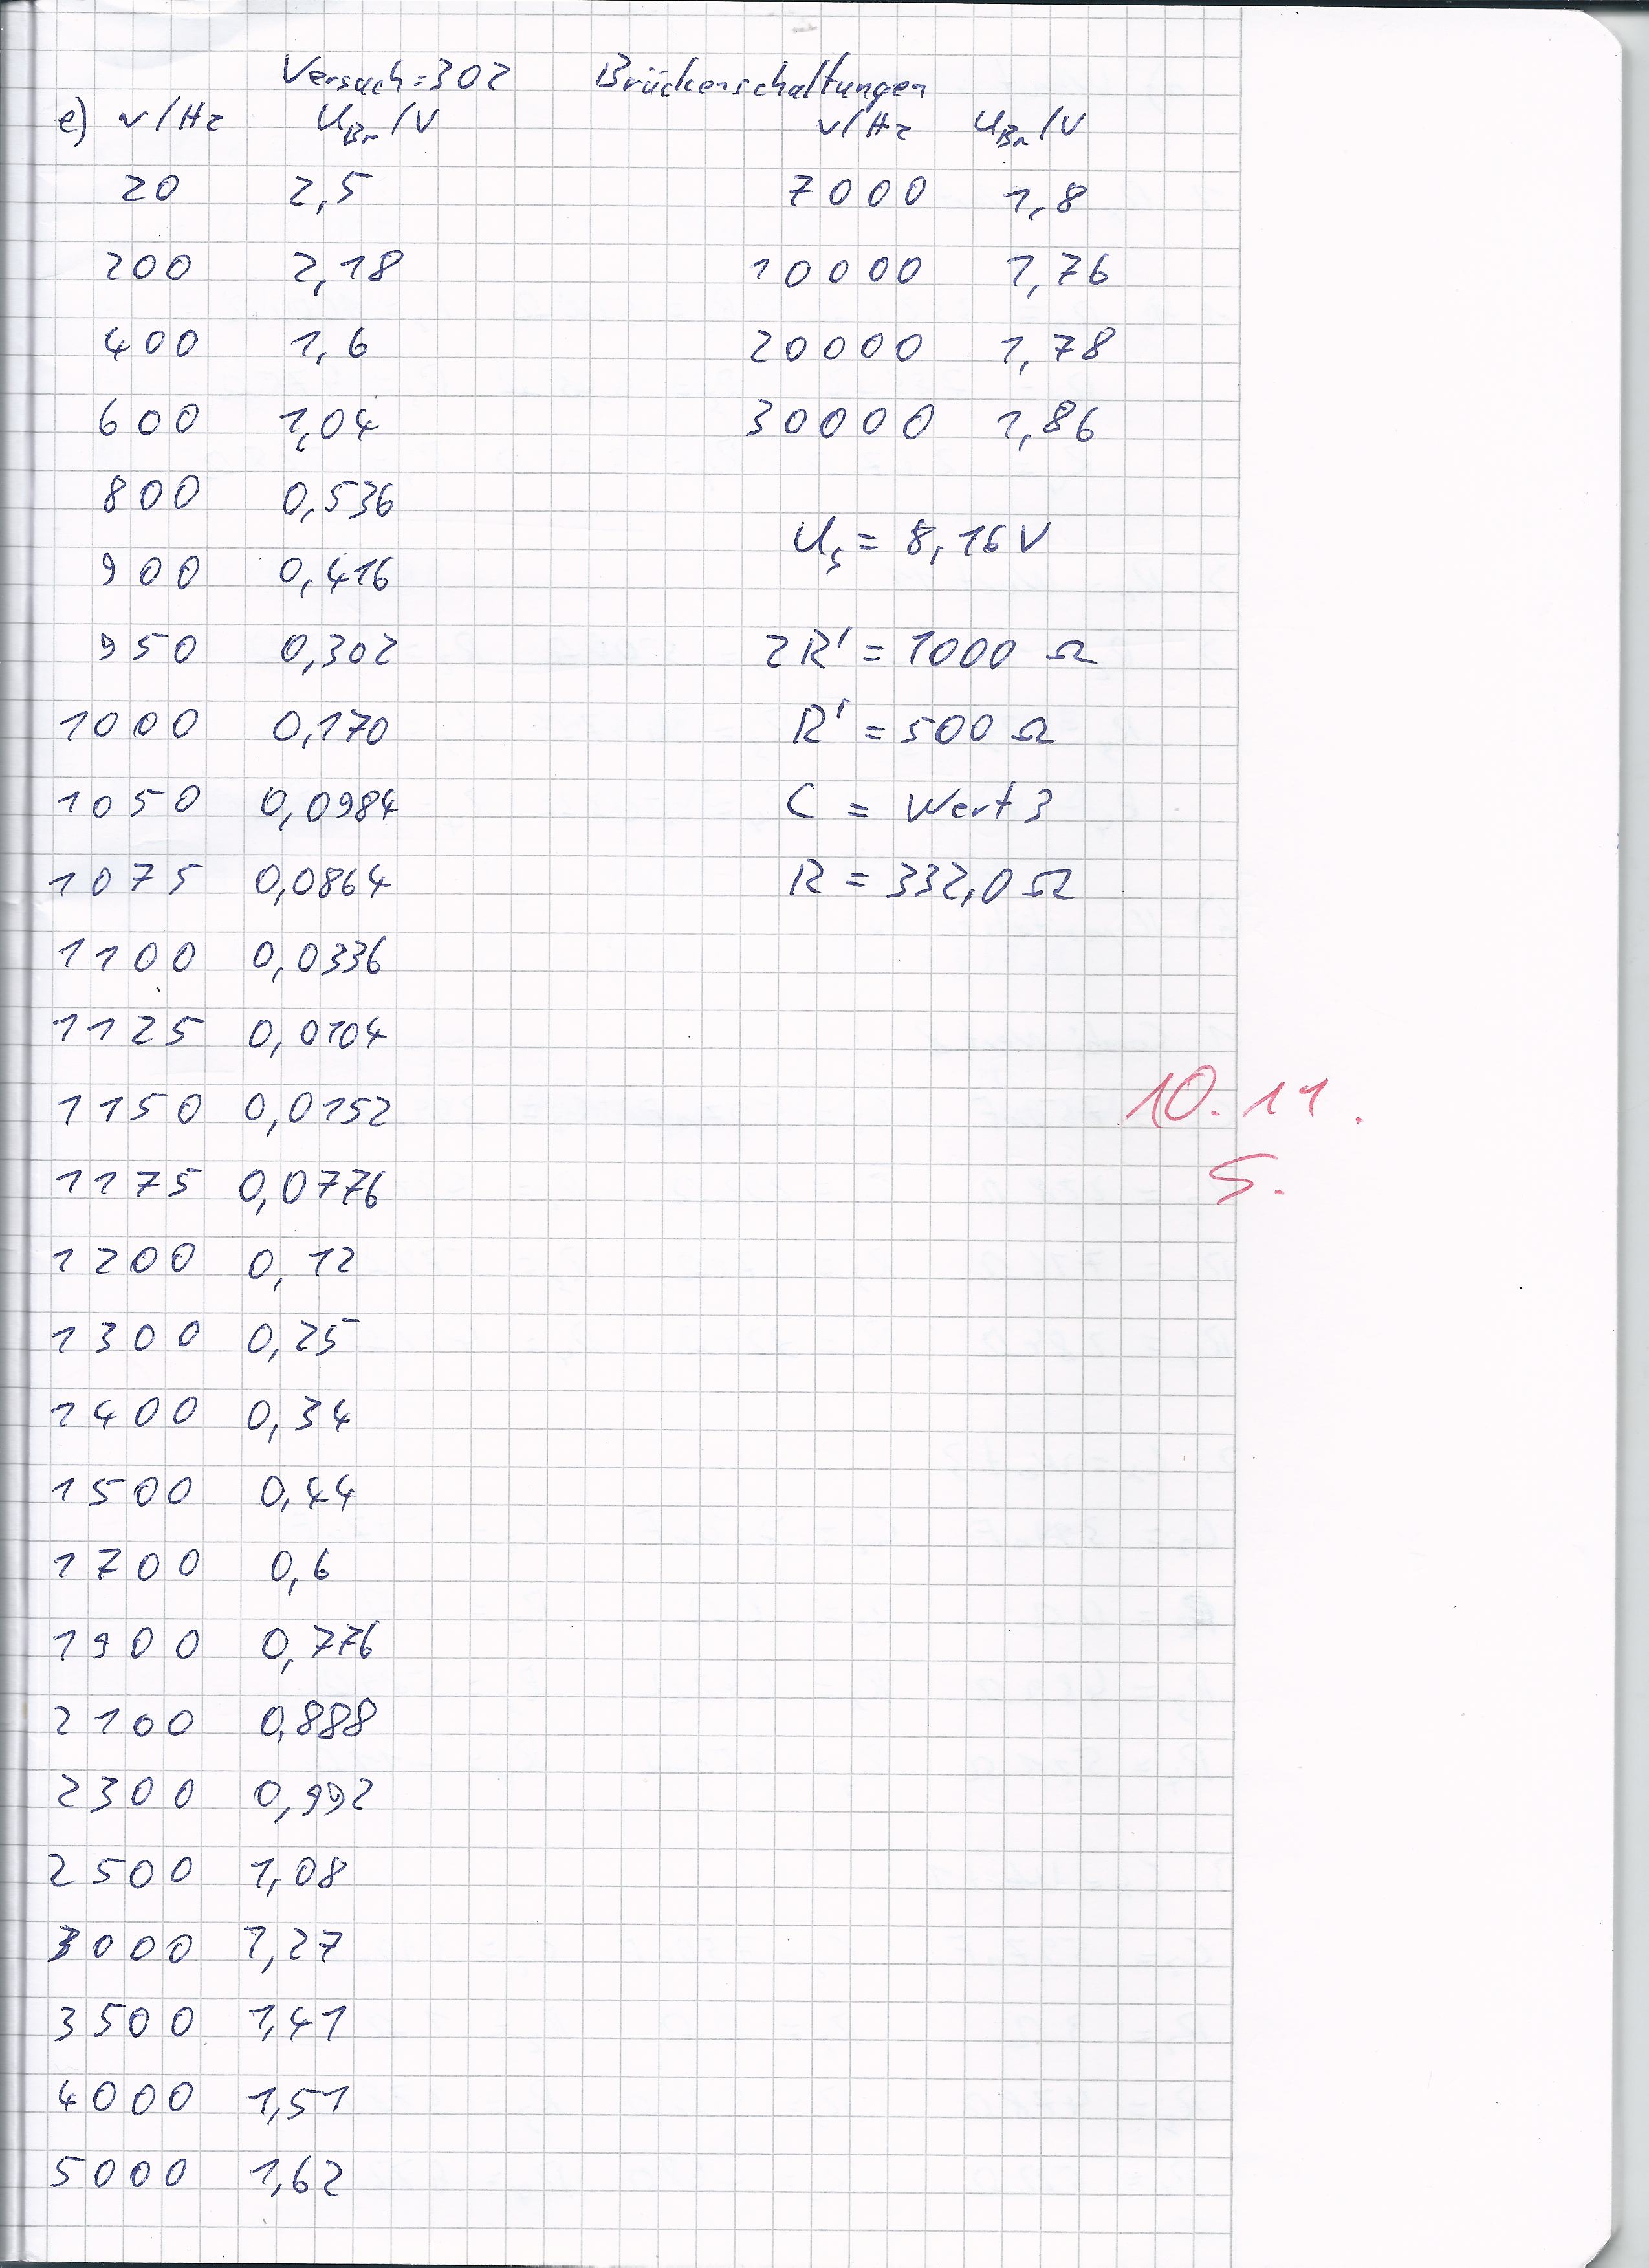
\includegraphics[height=14cm]{originaldaten-1.png}
  \caption{Originaldaten Teil 1.}
  \label{fig:original1}
\end{figure}

\begin{figure}[H]
  \centering
  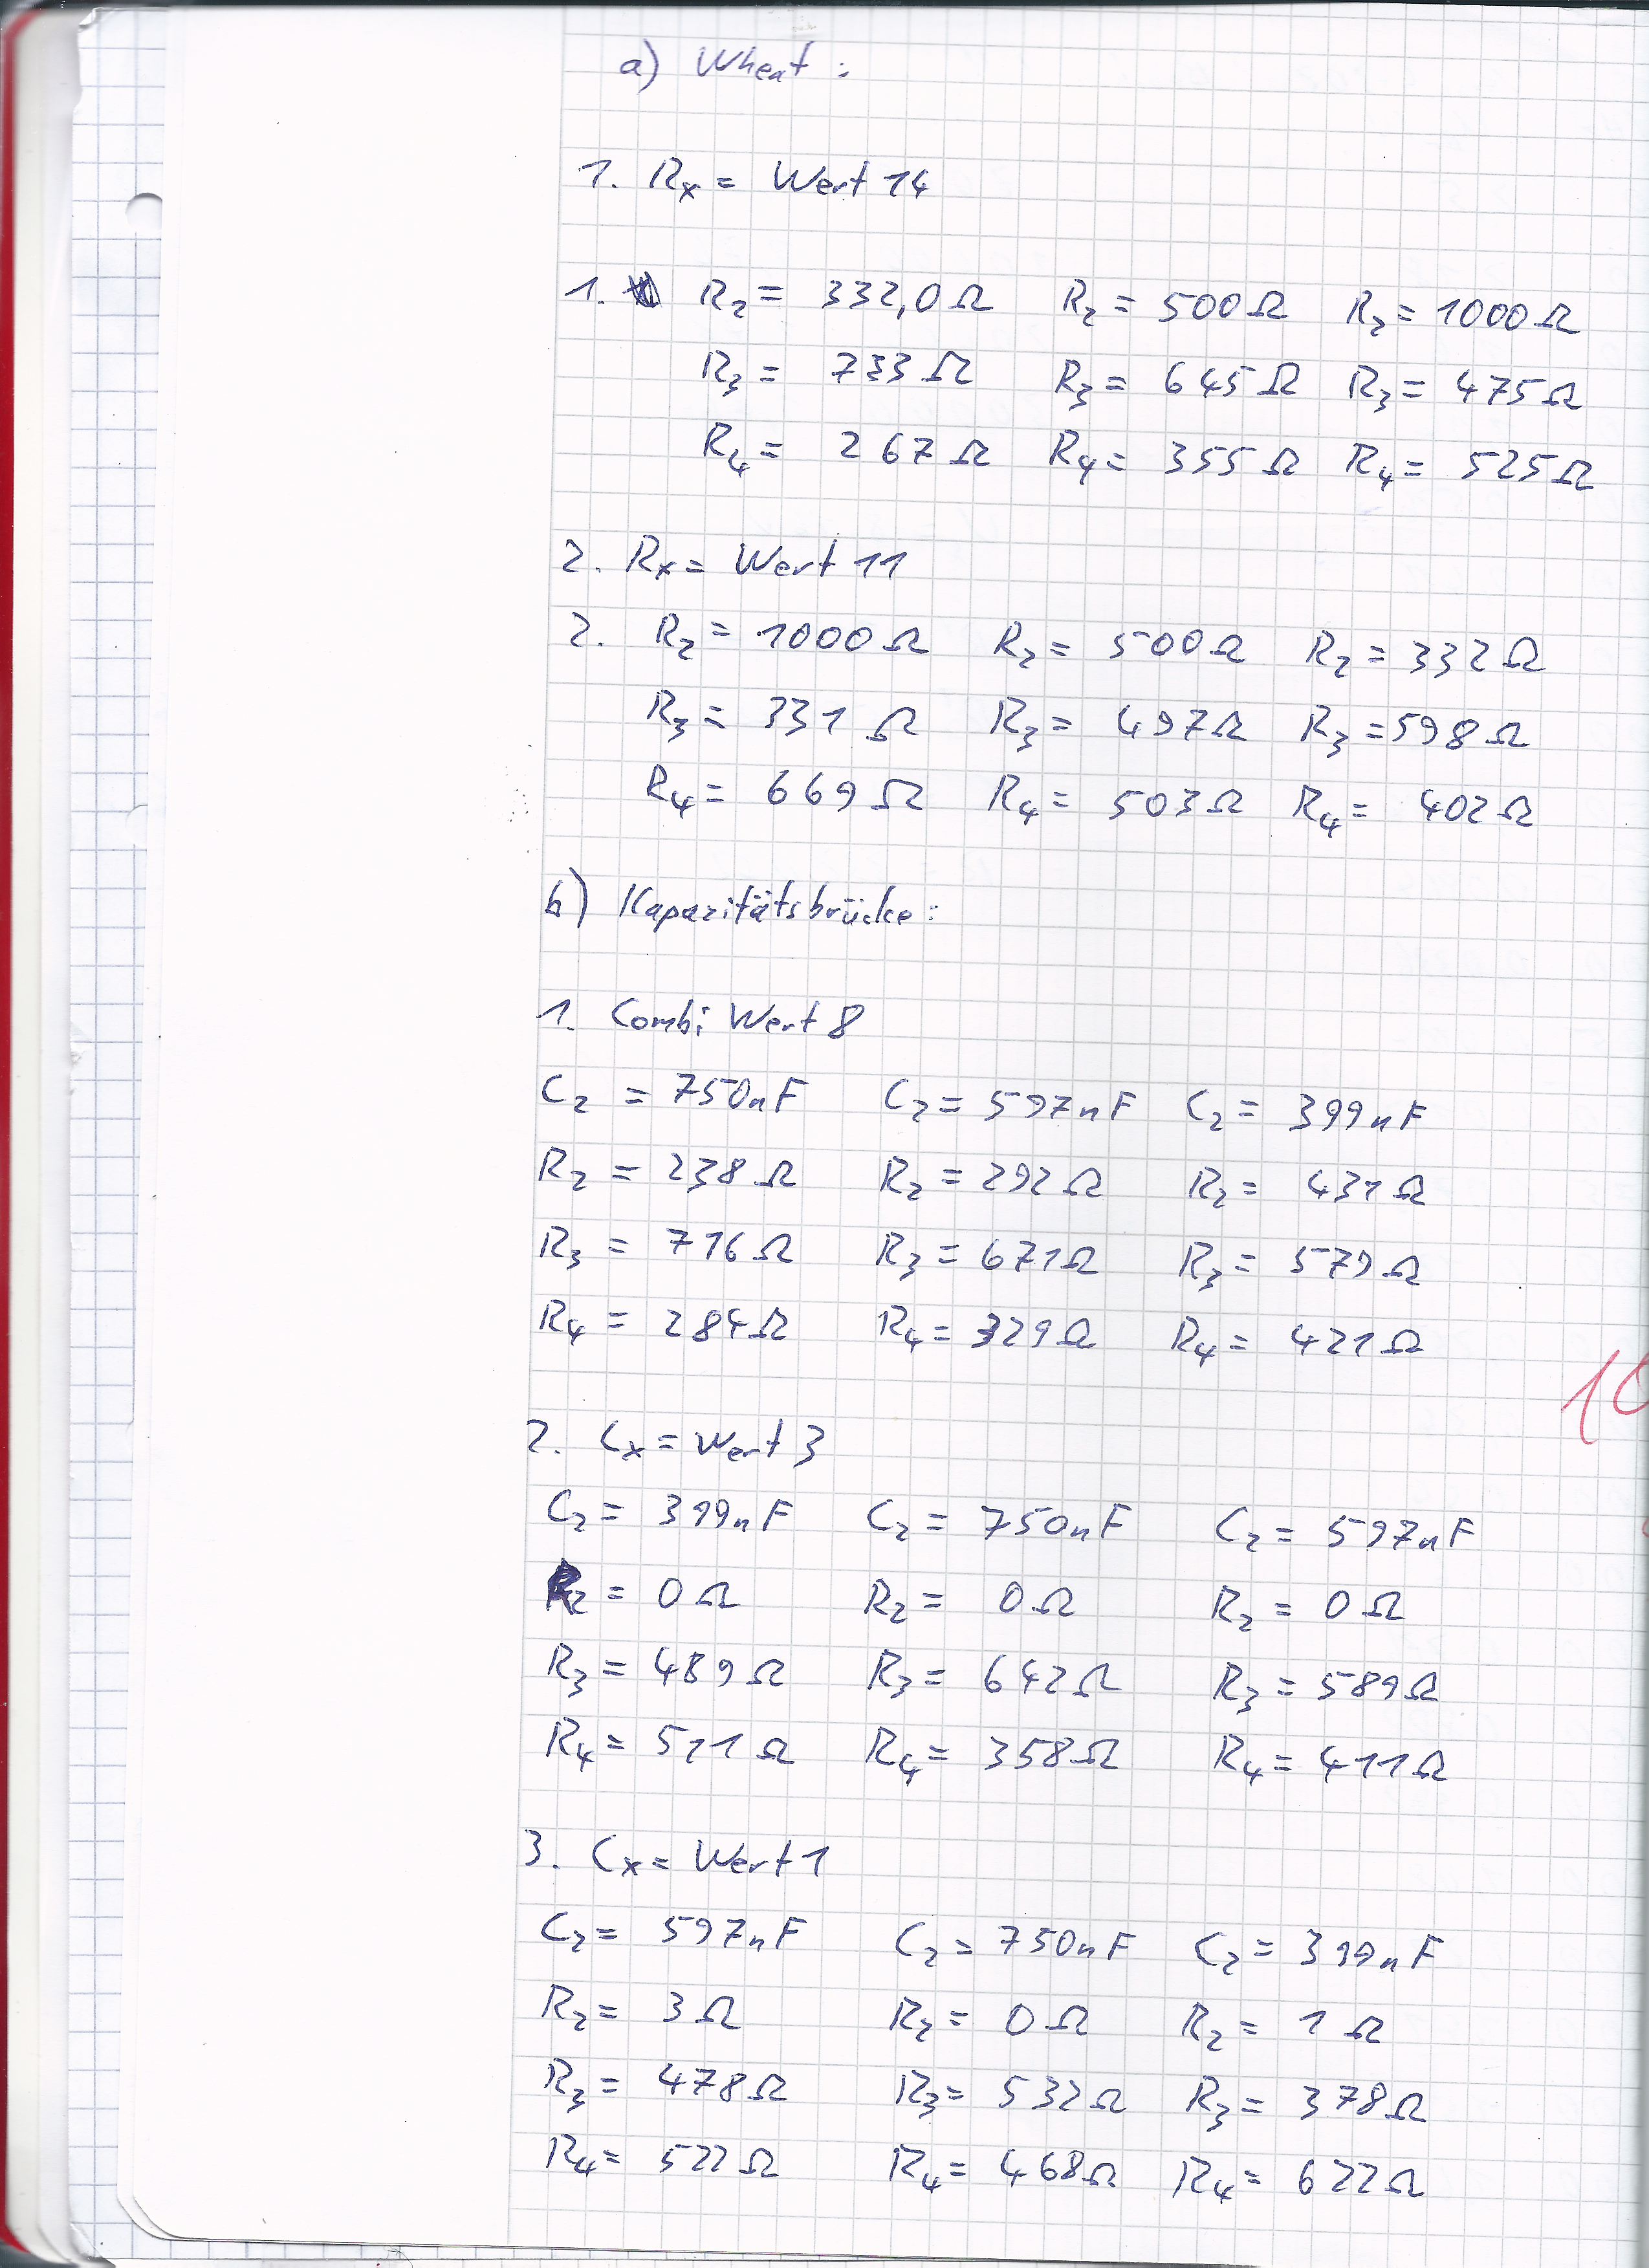
\includegraphics[height=14cm]{originaldaten-2.png}
  \caption{Originaldaten Teil 2.}
  \label{fig:original2}
\end{figure}

\begin{figure}[H]
  \centering
  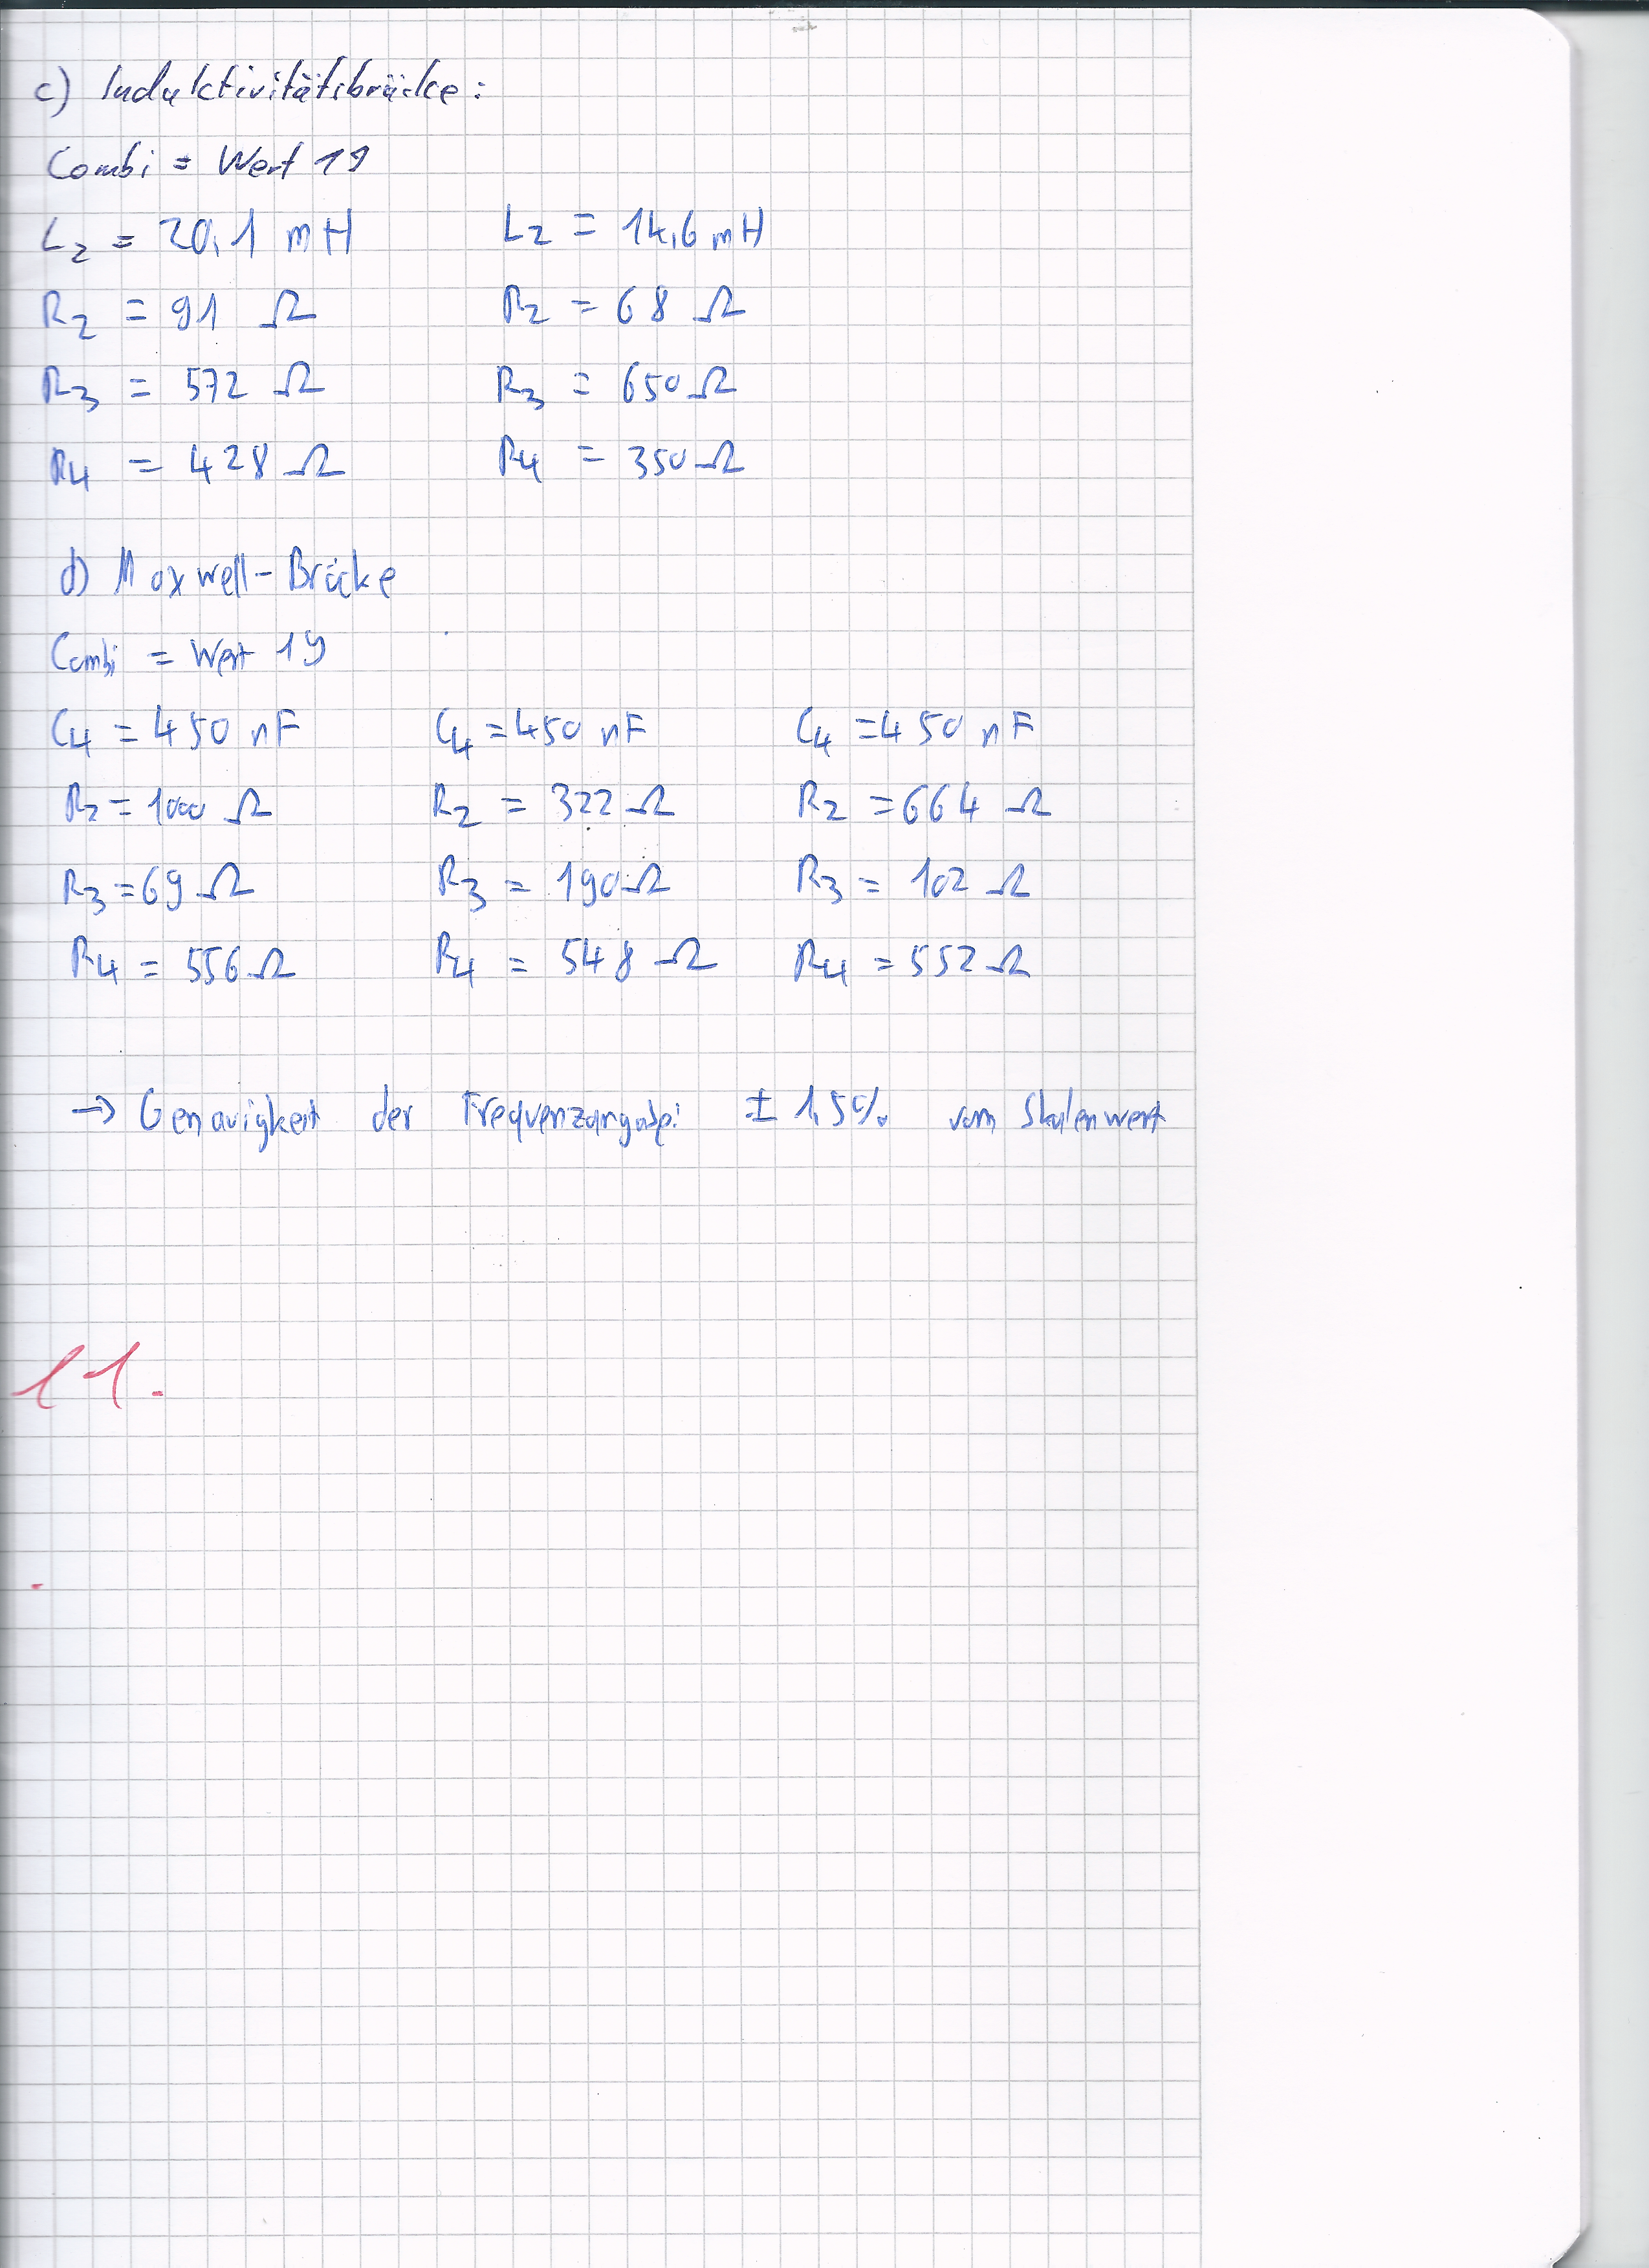
\includegraphics[height=14cm]{originaldaten-3.png}
  \caption{Originaldaten Teil 3.}
  \label{fig:original3}
\end{figure}

\printbibliography

\end{document}
